\documentclass[9pt]{beamer}
\usepackage{epstopdf}
\usepackage{etex}
\usepackage{pres}
\usepackage{gensymb}
\usetikzlibrary{patterns}

\makeatletter
\newif\if@restonecol
\makeatother
\let\algorithm\relax
\let\endalgorithm\relax
\usepackage[ruled,vlined,linesnumbered,lined]{algorithm2e}

\usefonttheme[onlymath]{serif}

\newcommand{\sseq}[1]{{\color{blue}\seq{#1}}}

\newcommand{\poly}{\textrm{poly}}
\newcommand{\Rat}{\mathbb{Q}}

\providecommand{\DontPrintSemicolon}{\dontprintsemicolon}

\pgfdeclareimage[width=6cm]{cps}{cps}

\hypersetup{
  pdftitle={Formal Verification: Projects},
  pdfauthor={Umang Mathur}}

\title{An Optimization Approach for Solving Reachability in Cyber-Physical Systems}
\author{Umang Mathur \and Atul Sandur}
  

\institute[CS, UIUC] {\vspace{0.1cm} 
  Department of Computer Science\\
  University of Illinois, Urbana Champaign} 

  
\date{\today}

%%%%%%%%%%%%%%%%%%%%%%%%%%%%%%%%%%%%%%%%%%%%%%%%%%%%%%%%%%%%%%%%%%%%%%%%%%%%%%%%%%%%%%%%%% 
%%    Main Body
%%%%%%%%%%%%%%%%%%%%%%%%%%%%%%%%%%%%%%%%%%%%%%%%%%%%%%%%%%%%%%%%%%%%%%%%%%%%%%%%%%%%%%%%%%

\begin{document}

\frame{\titlepage}

\frame{\frametitle{Outline}
\tableofcontents}

\section{Introduction}

\subsection{Cyber-Physical Systems}
 \frame{
  \frametitle{Cyber-Physical Systems (CPS)}
  \pause
  \begin{itemize}
    \item Cyber-Physical systems are engineered systems that depend upon the integration of \pause
        \begin{itemize}
            \item computational algorithms, and \pause
            \item physical components \pause
        \end{itemize}
    \vspace{0.25in}
    \item Diverse applications: \pause
        \begin{itemize}
            \item Healthcare : Pacemakers, Robotic arms\pause
            \item Aerospace, Aeronautics : auto-pilots \pause
            \item Chemical processes : Controllers ofr checmical plants \pause
            \item Transportation : Self driving cars \pause
            \item Energy sector : Nuclear reactors 
        \end{itemize}
  \end{itemize}
}
   
\frame{
  \frametitle{Cyber-Physical Systems (CPS)}
  \begin{center}
    \pgfuseimage{cps} 
  \end{center}
}

\subsection{Hybrid Automata for Modelling CPS}

\frame{
  \frametitle{Hybrid Automata: Modelling, Analysis and Synthesis of CPS}
  \pause
  \begin{itemize}
  \item
    Introduced by Alur et al. to model hybrid systems \pause
  \item
    Quite expressive, but \blue{undecidable} verification (reachability)
    problems  \pause
  \item
    Decidable subclasses exists, e.g. \pause
    \begin{itemize}
    \item 
      \blue{Timed Automata} ({\footnotesize Alur, and Dill}), \pause
    \item 
      \blue{Initialized Rectangular Hybrid automata} ({\footnotesize Henzinger
        et al.}), \pause
 %   \item 
 %     \blue{Multi-Mode Systems} ({\footnotesize Alur, Trivedi, Wojtczak})   
    \end{itemize}
    \item Most verification techniques rely on exhaustive exploration of state space using finite bisimulations \pause
%  \item 
 %   \blue{Tool support}: \textsc{HyTech}, \textsc{PHAV}er, \textsc{Uppaal}
  \end{itemize}
  \pause
    \begin{figure}
  \begin{center}
    \scalebox{0.8}{
    \begin{tikzpicture}[->,>=stealth',shorten >=1pt,auto,semithick]
      \tikzstyle{every state}=[fill=blue!30,minimum size=3em,rounded rectangle]
      
      \node[state] at (0, 0) (m0) {$\begin{array}{c}
          \mbox{\bf Off} \\ \dot{T} = -0.1T \\ T \geq 18 \end{array}$};
      
      \node[state] at (7, 0) (m1) {$\begin{array}{c} \mbox{\bf On} \\ \dot{T} = 5-0.1T \\ T \leq 22 \end{array}$};
     % \pause
  
      \path (m0) edge[bend left] node {$T < 19$} (m1);
      
      
      \path (m1) edge[bend left] node {$T > 21$} (m0);
      %\path (m0) edge node[] {$x_2 > 0, b$} (m2);
      
      %\path (m2) edge node[] {$ x_1 < 22, c$} (m3);
      %\path (m1) edge node[] {$d$} (m3);
   
      %\path (m3) edge [loop above] node[] {$e$} (m3);
    \end{tikzpicture}
  }
\end{center}
\label{fig:sha}
  \caption{Modelling a smart heater as a Hybrid Automata} 
\end{figure}
 
}

\section{Verification of Hybrid Automata}
\frame{\tableofcontentscurrent}

\subsection{Reachability : Motivation}

\frame{
  \frametitle{Reachability in Hybrid Systems}
  \pause
  Safety Critical Systems : \pause
    \begin{itemize}
        \item Nuclear reactors \pause
        \item Chemical plants \pause
        \item Aeronautics/Automobile \pauses
    \end{itemize}
    It is therefore important to have certain safety guarantees for such systems \pause

    \vspace{0.2in}
    Checking reachability of certain states, thus, is a natural question to ask \pause
    \begin{itemize}
        \item Can reach some error state ? \pause
        \item How to reach ? \pause
            \begin{itemize}
                \item input ? \pause
                \item path ? (non-determinism) \pause
            \end{itemize}
    \end{itemize}

    \vspace{0.2in}
    Other interesting applications: \pause
    \begin{itemize}
        \item Motion planning 
    \end{itemize}
        
%%  \begin{center}
%%    \scalebox{0.8}{  \begin{tikzpicture}[node distance=1cm]
      \node[loc,label=below:$m_1$] (p4) at (0,-2.5) {$\begin{matrix} \dot{T_1} =
          -2 \\ \dot{T_2} = 3 \end{matrix}$};
      \node[loc,label=below:$m_2$] (p5) at (3,-2.5){$\begin{matrix} \dot{T_1} = -1 \\ \dot{T_2} = -1 \end{matrix}$};
    \node[loc,label=below:$m_3$] (p6) at (6,-2.5){$\begin{matrix} \dot{T_1} = -1 \\ \dot{T_2} = 3 \end{matrix}$};
    \node[loc,label=below:$m_4$] (p7) at (0,-5) {$\begin{matrix} \dot{T_1} = 2 \\ \dot{T_2} = -2 \end{matrix}$};
    \node[loc,label=below:$m_5$] (p8) at (3,-5){$\begin{matrix} \dot{T_1} = 2 \\ \dot{T_2} = -1 \end{matrix}$};
    \node[loc,label=below:$m_6$] (p9) at (6,-5){$\begin{matrix} \dot{T_1} = 2 \\ \dot{T_2} = 3 \end{matrix}$};
  \end{tikzpicture}
}
%%  \end{center}
%%  
%%  \vfill
%%
%%  \blue{Safe Schedulability Problem:} Does there exist a \blue{switching schedule} using these \blue{modes}
%%    such that the temperatures stay in \blue{comfortable region}? 
}

\subsection{Example}

\frame{
    \frametitle{Robotic Motion Planning}
    \pause
    
    \vspace{-0.2in}
    \begin{figure}%{l}{0pt}%[0.4\textwidth]
%\begin{center}
  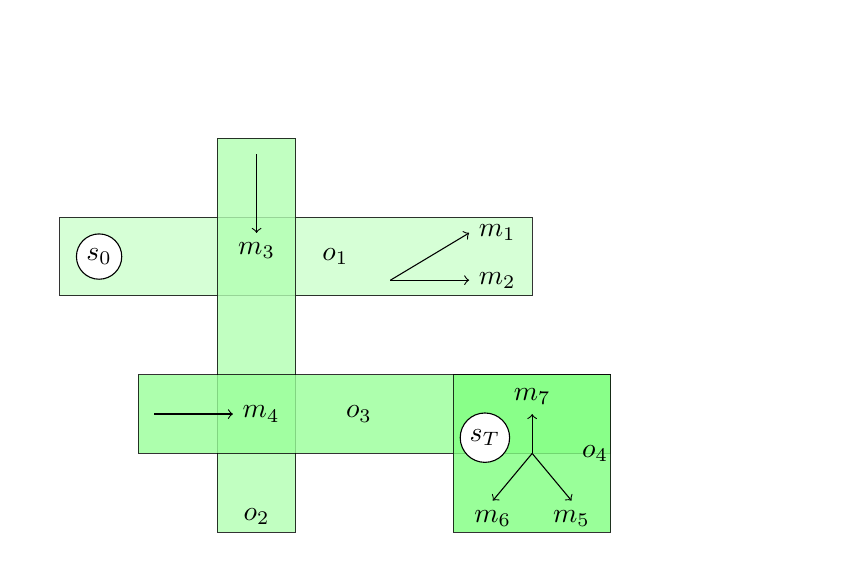
\begin{tikzpicture}
  \tikzstyle{every state}=[fill=gray!20!white,shape=rounded rectangle]
  
    \draw [fill=green!20, opacity=0.8] (0,0) rectangle (6,1);
    \node at (3.5, 0.5) {$o_1$};
    \node[fill=white!80, circle,inner sep=0.2em, draw] at (0.5, 0.5) {${\color{black}s_0}$};
    \draw[->] (4.2, 0.2) -- (5.2, 0.8) node[right] {$m_1$};
    \draw[->] (4.2, 0.2) -- (5.2, 0.2) node[right] {$m_2$};
    
    \draw [fill=green!30, opacity=0.8] (2,2) rectangle (3,-3);
    \node at (2.5, -2.8) {$o_2$};
    \draw[->] (2.5, 1.8) -- (2.5, 0.8) node[below] {$m_3$};
    
    \draw [fill=green!40, opacity=0.8] (1, -1) rectangle (7, -2);
    \node at (3.8, -1.5) {$o_3$};
    \draw[->] (1.2, -1.5) -- (2.2, -1.5) node[right] {$m_4$};
    
    \draw [fill=green!50, opacity=0.8] (5, -1) rectangle (7, -3);
    \node at (6.8, -2) {$o_4$};
    \draw[->] (6, -2) -- (6.5, -2.6) node[below] {$m_5$};
    \draw[->] (6, -2) -- (5.5, -2.6) node[below] {$m_6$};
    \draw[->] (6, -2) -- (6, -1.5) node[above] {$m_7$};
    \node[fill=white,circle,inner sep=0.2em, draw] at (5.4, -1.8)
    {${\color{black}s_T}$};
    
	\draw [dashed, draw=white] (6.6, 1.4) rectangle (7.4, -0.4);
    \draw [dashed, draw=white] (2.1, 3.4) rectangle (2.9, 2.6);
    \draw [dashed, draw=white] (-0.4, -1.1) rectangle (0.4, -1.9);
	\draw [dashed, draw=white] (7.6, -2.9) rectangle (9.9, -1.1);
      
  \end{tikzpicture}                        
%\end{center}
  \caption{Robotic motion planning problem modelled as a reachability question}
  \label{fig:robocop}
\end{figure}


    \begin{itemize}
        \item Can a bot enter $o4$ starting from some point in region $o1$ 
    \end{itemize}
}


\section{Singular Hybrid Automata}

\subsection{Syntax}

\frame{
	\frametitle{Syntax of SHA}
    \pause
    \begin{block}{Syntax : Singular Hybrid Automata (SHA)}
    \pause
	A singular hybrid automaton is a tuple
    \blue{$\Hh = (M, M_0, \Sigma, X, \Delta, I, F)$} 
    %\blue{$\Hh = (M, M_0, X, \Delta, I, F)$}
	where \pause
	\begin{itemize}
		\item $M$ is a finite set of control {\color{blue}{modes}} and $M_0 \subseteq M$,  \pause
		\item $\Sigma$ is a finite set of {\color{blue}actions}, \pause
		\item $X$ is a finite set of {\color{blue}variables},  \pause
		%\item $\Delta \subseteq M \times \poly(X) \times 2^{X} \times M$ is the {\color{blue}transition relation}, 
		\item $\Delta \subseteq M \times \poly(X) \times \Sigma \times 2^{X} \times M$ is the {\color{blue}transition relation},  \pause
		\item $I: M \to \poly(X)$  is the {\color{blue}mode-invariant} function, and \pause
		\item $F: M \to \Rat^{|X|}$ is the mode-dependent {\color{blue}flow function} characterizing the rate of each variable in each mode. \pause
	\end{itemize}
    \end{block}

    \begin{figure}
    \begin{center}
        \scalebox{0.8}{
            \begin{tikzpicture}[->,>=stealth',shorten >=1pt,auto,semithick]
                \node[loc, label=below:$m_0$, label=left:
                $\begin{matrix}
                    x_1 - 3x_2 \leq 10 \\
                    x_2 > -3
                \end{matrix}$] (m0) at (0,-2.5) {
                    $\begin{matrix}
                        \dot{x_1} = -2 \\ 
                        \dot{x_2} = 3 
                    \end{matrix}$
                };
                \node[loc,label=below:$m_1$, label=right:$2x_1 + 3x_2 \leq 5$] (m1) at (5,-2.5) {
                    $\begin{matrix}
                        \dot{x_1} = 0 \\ 
                        \dot{x_2} = -2
                    \end{matrix}$
                };
            
                \path (m0) edge[bend left] node {$a, \, x_1 + 2x_2 \leq 19$} node[below] {$\{x_2\}$} (m1);
                \path (m1) edge[bend left]  node[above] {$b, \, x_1 > -21$} node[below] {$\{x_1, x_2\}$}(m0);
            \end{tikzpicture}
        }
    \end{center}
    \label{fig:sha-syntax}
    \caption{Example SHA} 
\end{figure}

	
}

\subsection{Semantics}

\frame{
	\frametitle{Semantics of SHA}
    \pause
    \begin{block}{Semantics : Singular Hybrid Automata (SHA)}
    \pause
	\begin{itemize}
	\item \blue{Configuration} $(m, \nu)$, $m \in M$, $\nu \in \mathbb{R}^{\lvert X \rvert}$ \pause
    \item \blue{Timed action} $(t, a)$, $t \in \mathbb{R}^{\geq 0}$ and $a \in \Sigma$  \pause
	\item \blue{Transition} $((m, \nu) (t, a) (m', \nu'))$ \pause
%%%%	\begin{itemize}
%%%%        \item $(m, g, a, \mathcal{R}, m') \in \Delta$
%%%%            \begin{itemize}
%%%%                \item guard $g \in$ poly$(X)$
%%%%                \item $a \in \Sigma$
%%%%                \item reset set $\mathcal{R} \in 2^X$ 
%%%%            \end{itemize}
%%%%		\item For all $\hat{\nu} \in [\nu, \nu + t\cdot F(m)]$, $\hat{\nu} \in I(m)$ (Invariant)
%%%%        \item $\hat{\nu}' \in g$, where $\hat{\nu}' = \nu + t\cdot F(m)$
%%%%        \item   $\nu'(x_i)=
%%%%                    \begin{cases}
%%%%                        \nu(x_i) & x_i \not\in \mathcal{R}\\
%%%%                        0 & \text{ otherwise }
%%%%                    \end{cases}
%%%%                $
%%%%		\item $\nu' \in I(m')$ (Invariant)
%%%%	\end{itemize} 
	\item A \blue{run} is a sequence of transitions $(m_0, \nu_0) (t_1, a_1) (m_1, \nu_1) (t_2, a_2) \cdots$ \pause
	\end{itemize}
    \end{block}

    \begin{figure}
    \begin{center}
        \scalebox{0.8}{
            \begin{tikzpicture}[->,>=stealth',shorten >=1pt,auto,semithick]
                \node[loc, label=below:$m_0$, label=left:
                $\begin{matrix}
                    x_1 - 3x_2 \leq 10 \\
                    x_2 > -3
                \end{matrix}$] (m0) at (2.5,2.5) {
                    $\begin{matrix}
                        \dot{x_1} = -2 \\ 
                        \dot{x_2} = 3 
                    \end{matrix}$
                };
                \node[loc,label=below:$m_1$, label=right:$2x_1 + 3x_2 \leq 5$] (m1) at (7.5,2.5) {
                    $\begin{matrix}
                        \dot{x_1} = 0 \\ 
                        \dot{x_2} = -2
                    \end{matrix}$
                };
            
                \path (m0) edge[bend left] node {$a, \, x_1 + 2x_2 \leq 19$} node[below] {$\{x_2\}$} (m1);
                \path (m1) edge[bend left]  node[above] {$b, \, x_1 > -21$} node[below] {$\{x_1, x_2\}$}(m0);

            \pause 

            \only<8, 9, 12>{
                \node[yloc, label=below:$m_0$, label=left:
                $\begin{matrix}
                    x_1 - 3x_2 \leq 10 \\
                    x_2 > -3
                \end{matrix}$] (m0) at (2.5,2.5) {
                    $\begin{matrix}
                        \dot{x_1} = -2 \\ 
                        \dot{x_2} = 3 
                    \end{matrix}$
                };
            }

            \only<10, 11>{
                \node[yloc,label=below:$m_1$, label=right:$2x_1 + 3x_2 \leq 5$] (m1) at (7.5,2.5) {
                    $\begin{matrix}
                        \dot{x_1} = 0 \\ 
                        \dot{x_2} = -2
                    \end{matrix}$
                };
            }

    \node[stloc, label=left:
        $\begin{matrix} 
            x_1\\
            x_2
        \end{matrix}$,
        label=below:$m_0$] (s0) at (0,0) {$\begin{matrix} 0 \\ 0 \end{matrix}$};

    \pause
    \node[stloc, label=below:$m_0$] (s1) at (2,0) {$\begin{matrix} -2 \\ 3
      \end{matrix}$};  
    \draw[trans](s0) --node[midway,above]{$1$}  (s1);
    
    \pause
    \node[stloc, label=below:$m_1$] (s2) at (4,0) {$\begin{matrix} -2 \\ 0
      \end{matrix}$};  
    \draw[trans](s1) --node[midway,above]{$a$}  (s2);
    
    \pause
    \node[stloc, label=below:$m_1$] (s3) at (6,0) {$\begin{matrix} -2 \\ -1
      \end{matrix}$};  
    \draw[trans](s2) --node[midway,above]{$0.5$}  (s3);
    \pause
    \node[stloc, label=below:$m_0$] (s4) at (8,0) {$\begin{matrix} 0 \\ 0
      \end{matrix}$};  
    \draw[trans](s3) --node[midway,above]{$b$}  (s4);
    \draw[trans](s4) --node[midway,above]{$ \cdots$}  (10,0) ;


            \end{tikzpicture}
        }
    \end{center}
    \label{fig:sha-semantics}
    \caption{Example run in a SHA} 
\end{figure}

	
}

\subsection{Example}

\frame{
    \frametitle{Modelling Robot Motion Planning Using SHA}    

    \vspace{-0.2in}
    \begin{figure}%{l}{0pt}%[0.4\textwidth]
\begin{center}
  \begin{tikzpicture}
  \tikzstyle{every state}=[fill=gray!20!white,shape=rounded rectangle]
  
    \draw [fill=green!20, opacity=0.8] (0,0) rectangle (6,1);
    \node at (3.5, 0.5) {$o_1$};
    \node[fill=white!80, circle,inner sep=0.2em, draw] at (0.5, 0.5) {${\color{black}s_0}$};
    \draw[->] (4.2, 0.2) -- (5.2, 0.8) node[right] {$m_1$};
    \draw[->] (4.2, 0.2) -- (5.2, 0.2) node[right] {$m_2$};
    
    \draw [fill=green!30, opacity=0.8] (2,2) rectangle (3,-3);
    \node at (2.5, -2.8) {$o_2$};
    \draw[->] (2.5, 1.8) -- (2.5, 0.8) node[below] {$m_3$};
    
    \draw [fill=green!40, opacity=0.8] (1, -1) rectangle (7, -2);
    \node at (3.8, -1.5) {$o_3$};
    \draw[->] (1.2, -1.5) -- (2.2, -1.5) node[right] {$m_4$};
    
    \draw [fill=green!50, opacity=0.8] (5, -1) rectangle (7, -3);
    \node at (6.8, -2) {$o_4$};
    \draw[->] (6, -2) -- (6.5, -2.6) node[below] {$m_5$};
    \draw[->] (6, -2) -- (5.5, -2.6) node[below] {$m_6$};
    \draw[->] (6, -2) -- (6, -1.5) node[above] {$m_7$};
    \node[fill=white,circle,inner sep=0.2em, draw] at (5.4, -1.8)
    {${\color{black}s_T}$};

    \pause
    
	\node[state,fill=gray!20, scale=0.7] at (7, 1) (m1) {$m_1$};
	\node[state,fill=gray!20, scale=0.7] at (7, 0) (m2) {$m_2$};
	\draw [dashed] (6.6, 1.4) rectangle (7.4, -0.4);
	\path[->] (m1) edge[bend left] (m2);
     \path[->] (m2) edge[bend left] (m1);
	
	\node[state, fill=gray!20, scale=0.7] at (2.5,3) (m3) {$m_3$} ;
    \draw [dashed] (2.1, 3.4) rectangle (2.9, 2.6);
    
    \node[state, fill=gray!20, scale=0.7] at (0,-1.5) (m4) {$m_4$} ;
    \draw [dashed] (-0.4, -1.1) rectangle (0.4, -1.9);
    
	\node[state, fill=gray!20, scale=0.7] at (8,-1.5) (m5) {$m_5$} ;
	\node[state, fill=gray!20, scale=0.7] at (9.5,-1.5) (m6) {$m_6$} ;
	\node[state, fill=gray!20, scale=0.7] at (8.75,-2.5) (m7) {$m_7$} ;
	\draw [dashed] (7.6, -2.9) rectangle (9.9, -1.1);
	\path[->] (m5) edge (m6);
    \path[->] (m6) edge (m7);
    \path[->] (m7) edge  (m5);
      
    
    

  \end{tikzpicture}                        
\end{center}
  \caption{Robotic motion planning problem: Modelling as a SHA}
  \label{fig:robocop}
\end{figure}

}

\frame{
    \frametitle{Modelling Robot Motion Planning Using SHA}    

    \vspace{-0.2in}
    \begin{figure}[t]

  \begin{center}
     \scalebox{0.9}{
    \begin{tikzpicture}
      \tikzstyle{every state}=[fill=gray!20!white,minimum size=2em,shape=rounded rectangle]
      

      \node[state,fill=gray!20] (m1) {$m_1$};
      \node[state,fill=gray!20] at (0, -2) (m2) {$m_2$};
      \draw [dashed] (-0.5, 0.5) rectangle (0.5, -2.5) node[right] {$o_1$};
      \node at (0, -2.8) {$0{<} x {<} 6$};
      \node at (0, -3.1) {$0 {<} y {<} 1$};
      
      
      \node[state, fill=gray!20] at (2.5,0) (m3) {$m_3$} ;
      \draw [dashed] (2, 0.5) rectangle (3, -0.5) node[right]{$o_2$} ;
      \node at (2.5, -0.8) {$2{<} x {<} 3$};
      \node at (2.5, -1.1) {$-3 {<} y {<} 3$};

      \node[state, fill=gray!20] at (5.5,0) (m4) {$m_4$} ;
      \draw [dashed] (5, 0.5) rectangle (6, -0.5) node[right]{$o_3$};
      \node at (5.5, -0.8) {$1{<} x {<} 7$};
      \node at(5.5, -1.1) {$-2 {<} y {<} {-}1$};

      \node[state, fill=gray!20] at (8,0) (m5) {$m_5$} ;
      \node[state, fill=gray!20] at (10,0) (m6) {$m_6$} ;
      \node[state, fill=gray!20] at (9,-2) (m7) {$m_7$} ;
      \draw [dashed] (7.5, 0.5) rectangle (10.5, -2.5) node[right]{$o_4$};
      \node at (9, -2.8) {$5 {<} x {<} 7, -3 {<} y {<} -1$};

     \path[->] (m1) edge[bend left] node [right] {$\top$}  (m2);
     \path[->] (m2) edge[bend left] node [left] {$\top$}  (m1);

     \path[->] (m1) edge node [above] {$2 {<} x {<} 3$}  (m3);
     \path[->] (m3) edge node [above] {$-2 {<} y {<} -1$}  (m4);

     \path[->] (m4) edge node [above] {$5 {<} x {<} 7$}  (m5);

    \path[->] (m5) edge node [above] {$\top$}  (m6);
    \path[->] (m6) edge node [right] {$\top$}  (m7);
    \path[->] (m7) edge node [left] {$\top$}  (m5);
    \end{tikzpicture}
    }
  \end{center}
\caption{Singular Hybrid Automaton for robotic motion planning example}
\label{fig:wsha}
\end{figure}


}

\subsection{Reachability in SHA}

\frame{
  \frametitle{Reachability in SHA}
  \pause
  \begin{block}{Configuration Reachability Problem}
    Given a \blue{singular hybrid automaton $\mathcal{A}$}, a set of starting configurations $\mathcal{S}$, and a set of target configurations $\mathcal{T}$, decide whether there exists a
    \begin{itemize}
        \item \blue{finite} run 
        \item starting from some starting from some $(m, \nu) \in \mathcal{S}$, and
        \item ending in some $(m', \nu') \in \mathcal{T}$
    \end{itemize}
  \end{block}
\pause

  \vspace{0.4in}
  \begin{theorem}[Henzinger et. al., '98]
      Configuration reachability problem is undecidable for 3 or more continuous variables. 
  \end{theorem}
}

\section{Concolic walk}

\frame{
  \frametitle{Concolic Testing and Concolic Walk}
  \pause
  Concolic Walk \pause
    \begin{itemize}
        \item Concolic \pause = '\blue{conc}'rete evaluation  \pause + symb\blue{olic} reasoning \pause
        \item Ask an external solver to solve constaints (symbolic) \pause
        \item Use concrete values if solver cannot afford to solve (concrete) \pause
        \item Walk : \pause
        \begin{itemize}
            \item Quantify (fitness function) distance of actual solution from (half) state space (obtained from solvable constraints) \pause
            %\item Use fitness function to measure how close a point in half-space (obtained from linear constraints) is to global solutions for whole path condition
            \item Use search heuristics to guide random walk towards the goal (finding support of fitness function) \pause
        \end{itemize}
	\item Soundness guaranteed : No false alarms ! \pause
    \item Incomplete - Inherently undecidable
    \end{itemize}
}

\section{Our Approach}

\subsection{Understanding the Problem}

\frame{
  \frametitle{Problem in focus}
  \pause
    \begin{itemize}
        \item Given a 'symbolic' \blue{path}, checking for reachability is \blue{easy} \pause
        \begin{itemize}
            \item \blue{Simple} set of constraints \pause : Linear program \pause
            \item Check for feasibility \pause
        \end{itemize}

    \vspace{0.1in}
        \item Coming up with the right path : \blue{difficult} \pause
        \begin{itemize}
            \item Potentially infinite paths to be considered! \pause
            \item Problem is undecidable ! 
        \end{itemize}
    \end{itemize}
}

\subsection{Tackling the Problem}

\frame{
\frametitle{Generating Relevant Paths}
    \pause
    Quadratic programming and Search algorithms to the rescue ! \pause
    \vspace{0.1in}
    \begin{itemize}
        \item Every set of infeasible constraints from the symbolic path gives some information \pause
        \begin{itemize}
            \item How close it is to the target region \pause
            \item Use \blue{quadratic programming} :  
            \begin{equation*}
                \begin{array}{ll@{}ll}
                    \text{minimize}     & \|x-y \| &\\
                    \text{ } & & \\
                    \text{subject to}   & A_1 \: x \leq b_1\\
                    \text{and}          & A_2 \: y \leq b_2
                \end{array}
            \end{equation*}
            \pause
        \end{itemize}
        \item Search heuristics fo systematic exploration of paths: \pause
        \begin{itemize}
            \item Check if you are moving closer \pause
            \item If not, prune the search space \pause
            \item Otherwise, move even closer !
        \end{itemize}
    \end{itemize}
}

\subsection{Example}

\frame{
    \frametitle{Example : Search Guided Path Exploration}
        \definecolor{targetcolor}{rgb}{0.6,0.2,0}
    \definecolor{polycolor}{rgb}{1,0,0.2}
    \definecolor{gridcolor}{rgb}{0.75,0.75,0.75}
   % \begin{tikzpicture}[line cap=round,line join=round,>=triangle 45,x=1.0cm,y=1.0cm]
    \begin{tikzpicture}
            \begin{scope}[->,>=stealth',shorten >=1pt,auto,semithick, transform canvas={scale=0.6}, shift={(10,0)}]
                \node (dummyinit) at (1.5,2.5) {$\cdots$};
                \node[loc, label=below:$0 \leq y \leq 1 $] (m0) at (4,2.5) {
                    $\begin{matrix}
                        \dot{x} = 1 \\ 
                        \dot{y} = 2 
                    \end{matrix}$
                };
                \node[loc,label=below:$m_1$] (m1) at (8,2.5) {
                    $\begin{matrix}
                        \dot{x} = 1 \\ 
                        \dot{y} = 1
                    \end{matrix}$
                };
                \path (dummyinit) edge node[below] {$\{x, y\}$} (m0);
                \path (m0) edge[loop above] node[left] {$y \leq 1 \text{ }$} node[right] {$\text{ }\{y\}$} (m0);
                \path (m0) edge  node[above] {$x \geq 3$} (m1);

                \pause 

                \only<2,4,6,8,10,12>{
                \node[yloc, label=below:$0 \leq y \leq 1 $] (m0) at (4,2.5) {
                    $\begin{matrix}
                        \dot{x} = 1 \\ 
                        \dot{y} = 2 
                    \end{matrix}$
                };
                }

                \only<3,5,7,9,11>{
                \path (m0) edge[loop above, color=red] node[left] {$y \leq 1 \text{ }$} node[right] {$\text{ }\{y\}$} (m0);
                }


                \only<13>{
                \path (m0) edge[color=green]  node[above] {$x \geq 3$} (m1);
                }
            \end{scope}


        \begin{scope}[shift={(6,0)}, line cap=round,line join=round,>=triangle 45,x=1.0cm,y=1.0cm]
            \pgfmathsetmacro{\xoffset}{6.5}
            \draw [color=gridcolor,dash pattern=on 1pt off 1pt, xstep=0.5cm,ystep=0.5cm] (\xoffset-0.5,-1.5) grid (\xoffset+4.5,3.5);
            \draw[->,color=black] (\xoffset-0.5,0) -- (\xoffset + 4.5,0);
            \foreach \x in {0.5,1,1.5,2,2.5,3,3.5,4,4.5}
            \draw[shift={(\xoffset+\x,0)},color=black] (0pt,2pt) -- (0pt,-2pt) node[below] {\tiny $\x$};
            \draw[->,color=black] (\xoffset+0,-1.5) -- (\xoffset+0,3.5);
            \foreach \y in {-1.5,-1,-0.5,0.5,1,1.5,2,2.5,3,3.5}
            \draw[shift={(\xoffset,\y)},color=black] (2pt,0pt) -- (-2pt,0pt) node[left] {\tiny $\y$};
            \draw[color=black] (\xoffset-10pt, 2pt) node[right] {};

            \only<2>{
            \draw [line width=2pt, color=polycolor, shift={(\xoffset,0)} ] (0,0)-- (0.5,1);
            }

            \only<3>{
            \draw [line width=2pt, color=polycolor,  shift={(\xoffset,0)}] (0,0)-- (0.5,0);
            }

            \only<4>{
            \fill[line width=0pt,color=polycolor,fill=polycolor,fill opacity=0.25, shift={(\xoffset, 0)}] (0,0) -- (0.5,1) -- (1,1) -- (0.5,0) -- cycle;
            }

            \only<5>{
            \draw [line width=2pt, color=polycolor,  shift={(\xoffset,0)}] (0,0)-- (1,0);
            }

            \only<6>{
            \fill[line width=0pt,color=polycolor,fill=polycolor,fill opacity=0.25,  shift={(\xoffset,0)}] (0,0) -- (0.5,1) -- (1.5,1) -- (1,0) -- cycle;
            }

            \only<7>{
            \draw [line width=2pt, color=polycolor,  shift={(\xoffset,0)}] (0,0)-- (1.5,0);
            }

            \only<8>{
            \fill[line width=0pt,color=polycolor,fill=polycolor,fill opacity=0.25, shift={(\xoffset,0)}] (0,0) -- (0.5,1) -- (2,1) -- (1.5,0) -- cycle;
            }

            \only<9>{
            \draw [line width=2pt, color=polycolor,  shift={(\xoffset,0)}] (0,0)-- (2,0);
            }

            \only<10>{
            \fill[line width=0pt,color=polycolor,fill=polycolor,fill opacity=0.25, shift={(\xoffset,0)} ] (0,0) -- (0.5,1) -- (2.5,1) -- (2,0) -- cycle;
            }

            \only<11>{
            \draw [line width=2pt, color=polycolor, shift={(\xoffset,0)} ] (0,0)-- (2.5,0);
            }

            \only<12, 13>{
            \fill[line width=0pt,color=polycolor,fill=polycolor,fill opacity=0.25, shift={(\xoffset,0)} ] (0,0) -- (0.5,1) -- (3,1) -- (2.5,0) -- cycle;
            }

            \draw [color=targetcolor, shift={(\xoffset,0)} ] (3,3.5)-- (3,-1.5);
            \fill[pattern color=targetcolor, fill=targetcolor, pattern=north east lines, shift={(\xoffset,0)} ] (3,3.5) -- (4.5,3.5) -- (4.5,-1.5) -- (3,-1.5) -- cycle;
        \end{scope}

    \end{tikzpicture}

}

\section{Summary and Future Work}
\frame{
	\frametitle{Summary and Future Work}
\pause
    Summary \pause
    \begin{itemize}
        \item Systematic approach for solving reachability \pause
        \item Convex optimization \pause
        \item Heuristic search techniques \pause
        %\item <talk about tool> \pause
        %\item <talk about its performance> \pause
        %\item <talk about bottlenecks in performance> \pause
    \end{itemize}

    \vspace{0.1in}
    Future Work \pause
	\begin{itemize}
	\item Better Heuristics for Search \pause
        \item Techniques to prune exploration of paths of given length
        \item Proving properties about reachable sets : Monotonicity and Regularity \pause
        \item Use of abstractions : \pause
            \begin{itemize}
                \item Underapproximations of reachable sets to conservatively estimate the fitness function \pause
                \item Efficiently calculate the fitness function \pause
            \end{itemize}
        \item Extend approach for attacking loops in software programs
	\end{itemize}
}

\frame{
\frametitle{}
	\begin{center}

        \font\endfont = cmss9 at 15.40mm
        \endfont 
        \baselineskip 20.0mm

        Thank You !

      \end{center}    
}



%\nocite{*}

%\bibliographystyle{plain}
%\bibliography{papers}

\end{document}
